% Chapter X

\chapter{Extracting biological signal from contact maps} % Chapter title

\label{ch:02-01} % For referencing the chapter elsewhere, use \autoref{ch:name} 

%----------------------------------------------------------------------------------------

Most genomics methods generate a large amount of information, most of which is not directly relevant for the problem at hand. One of the main challenges emanating from genomics data is to distill this information and extract only the relevant signal.

In the case of Hi-C and other 3D genomics techniques, the resulting signal is a collection of contacts recorded between pairs of genomic regions. These contacts reflect the average genome structure from a population of cells and are subject to various biases.

The spatial features and changes of interest are diluted in the population and can be obfuscated by noise. Detecting these changes requires a set of bias correction and signal detection methods which are still in their early developments.

In this section we review the recent methodlogical developments that allow to correct the Hi-C signal and present new methods to extract biological features from these datasets. These developments proved necessary to tackle the questions raised in further chapters.

\section{Streamlined and reproducible Hi-C processing}
\label{sec:02-01:streamlined-processing}
% Existing methods: painful to install, non tested (risky), non reproducible
% hicstuff, hicreppy

Pre-processing of Hi-C data, to convert \acrfull{NGS} reads into chromosomal contact matrices involves several steps that will impact the resulting signal. The sequencing reads themselves can be the result from religation of two distinct loci (Fig. \ref{fig:02-01:chimeric}). These chimeric reads cannot be aligned reliably with generic methods and need to be cut for proper alignment. Chimeric reads become more problematic when increasing the read size relative to restriction fragment length.

\begin{figure}[htb]
    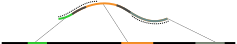
\includegraphics[width=0.8\textwidth]{Parts/Part02/gfx/hicstuff/chimeric.pdf}
    \caption{Chimeric reads in Hi-C: Example of a Hi-C fragment resulting in a chimeric read. The Hi-C fragment contains 3 different regions (green, orange and grey) which have been religated together. The paired-end sequencing reads are shown as dotted line. The sequencing read spanning the green and orange region will be chimeric and not map to a unique region.}
    \label{fig:02-01:chimeric}
\end{figure}

Not all read pairs generated by Hi-C experiments represent valid spatial interactions. Some restriction fragments are sequenced without religation and other fragments religate on themselves (Fig. \ref{fig:02-01:filters}). The various interaction types can be separated based on the strand of origin of their individual reads. In theory, and in practice at long ranges, one would expect religations to be strand agnostic and to have an equal represenation of all four possible combinations (++, --, +-, -+). In reality, this is never the case at short range contacts, due to the enrichment of self-religation (-+) and dangling ends (or undigested fragments, +-) \cite{cournacNormalizationChromosomalContact2012}.

\begin{figure}[htb]
    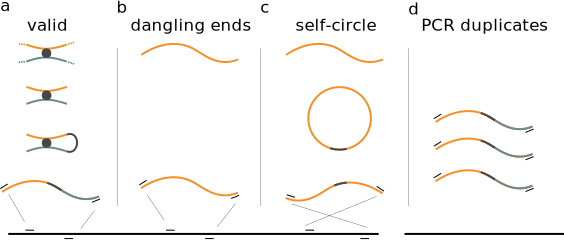
\includegraphics[width=\textwidth]{Parts/Part02/gfx/hicstuff/filters.pdf}
    \caption{Type of interactions generated from Hi-C experiments: \textbf{a:} Valid interaction resulting from the religation of two distant loci in physical contact. \textbf{b:} Spurious interaction caused by the sequencing of a single restriction fragment, or undigested sequence. \textbf{c:} Spurious interaction resulting from the self-religation and breakage of a fragment. \textbf{d:} Interactions caused by PCR duplicates. Both reads have the exact same coordinates for all PCR duplicate pairs.}
    \label{fig:02-01:filters}
\end{figure}

These biases must be accounted when processing Hi-C data. This can be achieved by identifying and filtering out faulty interactions based on their strands.

This preprocessing is often performed using custom scripts and prone to errors, bugs and lack of informations about parameters. In an effort to improve reproducibility and accessibility of Hi-C analysis, we developed hicstuff, an open source Hi-C pipeline that incorporate all the aforementioned steps, along with several downstream processing utilities (Fig. \ref{fig:02-01:pipeline}).

\begin{figure}[htb]
    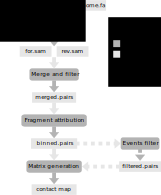
\includegraphics[width=0.7\textwidth]{Parts/Part02/gfx/hicstuff/pipeline.pdf}
    \caption{Overview of the hicstuff pipeline: Consecutive steps towards the generation of a contact map from sequencing reads, along with the intermediate files are shown as a directed acyclic graph.}
    \label{fig:02-01:pipeline}
\end{figure}

Hicstuff can properly align chimeric reads, by digesting them \textit{in-silico} at religation sites, or using iterative mapping (Fig. \ref{fig:02-01:iteralign}) where reads are truncated and iteratively extended until they align unambiguously. The Hi-C pairs are then assigned a numerical index according to the restriction they originate from (Fig. \ref{fig:02-01:attribution}) and artifactual contacts are filtered out using the strand information. Contacts in each bin combination are then summed into a "contact matrix", which is stored in sparse format to spare memory. To allow compatibility with various programs, it can generate sparse matrices in 3 possible formats (COO, bedgraph2d and cool).

\begin{figure}[htb]
    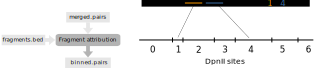
\includegraphics[width=0.8\textwidth]{Parts/Part02/gfx/hicstuff/hic_pipeline_attribution.pdf}
    \caption{Fragment attribution of Hi-C contacts: The genome is segmented into discrete bins according to the positions of restriction sites. Hi-C reads are assigned an index according to the restriction fragment to which they aligned.}
    \label{fig:02-01:attribution}
\end{figure}

\begin{figure}[htb]
    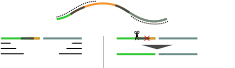
\includegraphics[width=1\textwidth]{Parts/Part02/gfx/hicstuff/iteralign.pdf}
    \caption{Iterative alignment of a Hi-C pair: The Hi-C fragment consists of 3 regions religated together (top). One sequencing read spans two regions (orange and green). Iterative alignment is used to uniquely align the resulting chimeric read (left). The read is truncated to a short length (e.g. 20bp) and iteratively extended until it aligns to a unique position in the genome. Alternatively, reads which do not map uniquely can be digested \textit{in-silico} at known religation sites (right) to remove the chimeric part. The digested reads are then realigned.}
    \label{fig:02-01:iteralign}
\end{figure}

\begin{figure}[htb]
    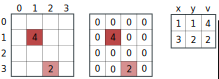
\includegraphics[width=\textwidth]{Parts/Part02/gfx/hicstuff/dense_sparse.pdf}
    \caption{Dense and sparse matrix representation: . In Hi-C, matrices are very sparse (i.e. mostly contain 0s), (left). In dense matrix representation, we store all values explicitely. The information stored is highly redundant (middle). Such matrices can be stored efficiently using a sparse representation where only non-zero values are stored explicitely along with their coordinates (right).}
    \label{fig:02-01:sparse}
\end{figure}

Hicstuff is meant to be easily accessible \cite{matthey-doretSimpleLibraryPipeline2021}, even to non-expert users. It has a comprehensive online documentation and tutorials and the program and its dependencies are installed with a single command. The code is written in python and is exposed both via a \acrfull{CLI} to use it as an executable, and an \acrfull{API} to import it as a python library. It is covered by unit tests which are automatically executed on each new release, on the cloud by a continuous integration service to reduce the likelihood of bugs. Hicstuff runs well with default parameters, but has many options to fit most common use cases. It works regardless of genome size organism.

The pipeline also provides reproducibility through an automatic logging of every intermediate result in the pipeline as well as the input parameters used.

The project has already fostered a modest community of users which are offering their contributions, suggest features or report issues they encounter.

\FloatBarrier
\section{Feature detection with Chromosight}

The downstream analysis of chromosome contact maps often involves looking for signals reflecting biologically relevant spatial interactions. Several specialized approaches for pattern detection have been proposed in the past. Each of these methods use a set of specific rules to detect one particular type of pattern. For example, HICCUPS \cite{rao3DMapHuman2014} detects chromatin loops by scanning each pixel of the contact map for contact enrichment compared to surrounding pixels.

These specialized methods present several drawbacks, including strong dependence on parameters, poor generalization to non-model species and poor detection rates. These shortcomings motivated us to work on a more generalized pattern detection method to identify arbitrary patterns in chromosome contact maps.

Chromosight uses template matching to identify features on a chromosome contact map. This technique consists in scanning the input Hi-C matrix with a smaller "kernel" image corresponding to the pattern of interest (e.g. a loop) to identify input regions bearing similarity to the kernel. This has the added benefit of allowing to swap the kernel to detect a different feature.

One of the main algorithmic challenges of applying a convolution-based method to Hi-C data is the size of matrices. Hi-C matrices are notoriously large, but they are also extremely sparse (loci do not interact with each other). As a consequence, sparse matrix representation is generally used to handle Hi-C data (Fig. \ref{fig:02-01:sparse}). In the case of large genomes, such as that of \textit{Homo sapiens}, this is necessary to store an entire chromosome's contact map into a regular computer's memory. One of the main drawbacks of sparse representation is that most algorithms are slower and harder to implement on such matrices. No implementation of convolution for sparse matrices was openly available, which prompted us to write an efficient method to scan the billion of pixels from Hi-C maps in reasonable time. Fortunately, the convolution problem can be reformulated as a matrix multiplication by transforming the input matrices (see \ref{sec:04-A-01:convolution}), and matrix multiplication is a standardized operation that has been highly optimized in low level libraries, including for sparse matrices.

Chromosight is a python package that takes cool files as input. During its development, we put special attention on good software practice mentioned in section \ref{sec:02-01:streamlined-processing} to make it easy to use and accessible. This was done by spending time documenting the python \acrshort{API} and the \acrshort{CLI} as well as putting tutorial examples. Furthermore, the program is covered by a suite of unit tests set up with continuous integration. On every new release, Chromosight is automatically distributed on PyPI, bioconda and dockerhub to accomodate the different use cases and pipelines.

Chromosights algorithm, results and benchmark against state of the art loop detection methods are presented in details in the following pages. The algorithmic details used to tackle the sparse convolution problem are presented in section \ref{sec:04-A-01:convolution}.

\includepdf[pages=-,addtotoc={
     2,subsection,2,Introduction,p1,   
     3,subsection,2,Results,p2,
     8,subsection,2,Discussion,p3,
     8,subsection,2,Methods,p4,
     12,subsection,2,Supplementary information,p5}]
     {Publications/chromosight_publication_supp.pdf}    

\section{Change detection across biological conditions}

Change detection is a common issue in the field of signal processing and remote sensing. Given two or more input signals such as images, we want to find portions that differ between the two inputs. This principle can also be applied to Hi-C contacts, where we can detect regions of contact maps that differ between biological conditions.

Change detection in Hi-C contact maps is required whenever we want to identify genomic regions whose spatial organization is altered between two conditions.

Many approaches can be taken to detect these changes. Some of them, such as diffhic, formulate the problem similarly to a differential expression RNAseq analysis using contact counts instead of read counts. This approach has the benefit of being straightforward, but it only finds contact increase. Local increase in contacts can represent a specific spatial interactions, but also differential accessibility or insulation. which could be caused by a number of different phenomena.

We developed pareidolia, a software package for change detection with an apriori on the type of signal to detect. The method is "supervised" in the sense that it requires a kernel representing the feature of interest. Pareidolia relies on Chromosight's backend to convert the contact map of each condition into a map of correlation coefficients representing similarity with the feature of interest. Change detection is then performed on these coefficients. As a consequence, rather than looking for contacts increase, pareidolia looks for changes in feature intensity, such as border sharpness or looping intensity.

\subsection{Pareidolia algorithm}

Pareidolia works by comparing one or several samples issued from two conditions such as treatments or timepoints.

Assuming two conditions $t={t_0, t_1}$, where multiple samples (replicates) $(r_1, r_2, ..., r_R)$ can share the same condition. The contact matrix from each sample $H_{r, t}$ is first convoluted with a kernel $K$ representing the pattern of interest, using Chromosight's \acrshort{API}. In the resulting matrix $M$, each value $M_{r, t}[i, j]$ is a Pearson correlation coefficient with the kernel. $M$ is computed as described in equation

Change detection can then be performed on the correlation maps using two different methods.

The first method is inspired by median filtering-based background formation (Fig. \ref{fig:02-01:pareidolia}). We generate a background matrix for each condition (timepoint), whose values are defined as the median of all replicates' correlation matrices from that condition (Eq. \ref{eqn:02-01:pareidolia-bg}) 

\begin{equation}
    \label{eqn:02-01:pareidolia-bg}
    B_t[i, j] = median(M_{1, t}[i, j], M_{2, t}[i, j], ..., M_{R, t}[i, j])
\end{equation}

We then compute the matrix of squared errors $V$ between each replicate and their condition's median background (Eq. \ref{eqn:02-01:pareidolia-sse}). This technical variability (among replicates) is then used to filter out noisy regions. This is done by generating a \acrfull{SNR} map $S$ (Eq. \ref{eqn:02-01:pareidolia-snr}) and applying a threshold to it.

\begin{align}
    \label{eqn:02-01:pareidolia-sse}
    V_t &= \sum_{i=1}^r{(M_{i, t} - B_t)^2} \\
    \label{eqn:02-01:pareidolia-snr}
    S &= \frac{1}{t} \sum_{i=0}^t{\frac{B_i}{V_i}}
\end{align}

Pixels in noisy regions (below the \acrshort{SNR} threshold) are then removed. To further reduce false detections, a density filter can be applied to discard detections located in low coverage regions. If a kernel of size $K$ was used for detection, the proportion of nonzero values within a window of size $K$ surrounding each position must be above a threshold to be considered.

\begin{figure}[htb]
    \includegraphics[width=\textwidth]{Parts/Part02/gfx/pareidolia_process.pdf}
    \caption{Pareidolia algorigthm. From top to bottom: The Hi-C contact maps of several replicates in two conditions are shown, as well as the difference between conditions. Chromosight's convolution algorithm is used on each sample (1) to generate a map of correlation coefficient with the kernel of interest (loops in this case). For each condition, a median background is computed among replicates (2). The difference between these two background is then extracted (3) and filtered (4) using a \acrshort{SNR} threshold and a percentile threshold.}
    \label{fig:02-01:pareidolia}
\end{figure}

Pareidolia can either return the change intensity on a set of predetermined loop positions provided as input, or perform \textit{de-novo} detection of differential loops on the Hi-C map. For detection, pareidolia uses Chromosight's implementation of the connected component labelling algorithm for sparse matrices.

\subsection{Results on experimental data}

To showcase the performances of Pareidolia, we used it to measure loop changes upon depletion of CTCF in murine cells \cite{noraTargetedDegradationCTCF2017}. CTCF acts as a roadblock for the motor protein cohesin which travels along the chromatin fiber. Cohesin accumulates at CTCF binding sites which forms stable chromatin loops between pairs of CTCF binding sites.

These looping interactions have been shown to disappear in the absence of cohesin \cite{raoCohesinLossEliminates2017} or CTCF \cite{noraTargetedDegradationCTCF2017}. Here we show an example use of Pareidolia to quantify these 3D changes.

\begin{figure}[htb]
    \includegraphics[width=\textwidth]{Parts/Part02/gfx/pareidolia/ctcf_depletion_comparison_maps_chr1_55Mb.pdf}
    \caption{Pareidolia results on CTCF degradation experiments from \cite{noraTargetedDegradationCTCF2017}: Blue circles indicate detection of differential loops between the two conditions.}
    \label{fig:02-01:pareidolia-experimental}
\end{figure}